\documentclass{article}
\usepackage{algorithmicx}
\usepackage{algpseudocode}
\usepackage{graphicx}
\usepackage{color}
\usepackage[utf8]{inputenc}


\begin{document}
{\noindent \Huge Problema a resolver: Plan de Vuelo}\newline  \newline

Se cuenta con una cantidad n, entero no negativo, de vuelos disponibles. Cada vuelo se realiza de una ciudad a otra, y para cada uno se conoce la hora de salida y la hora de llegada respectivamente.
 El objetivo del problema es que dadas dos ciudades por ejemplo: X (origen) e  Y (destino).  Se devuelva un itinerario con los vuelos necesarios para llegar desde origen a destino, siempre que sea posible.  De esta manera el primer vuelo que realice el itinerario devuelto debe ser desde X, y el último debe tener como lugar de llegada a Y. Para efectuar este recorrido es posible tomar cualquier cantidad de vuelos intermedios cuya combinación me permita llegar a destino. Pero, siempre que entre los vuelos elegidos, el horario de  llegada a una ciudad y el horario del próximo vuelo que se efectué  desde la misma, haya como mínimo dos horas de diferencia (el horario de salida y de llegada es la cantidad de horas que faltan para realizar cada una de las acciones desde el momento en que se realiza la consulta). 
Se considerada solución óptima del problema a aquel itinerario que cumpla con lo descripto pero además, en el itinerario devuelto la llegada a destino se realice lo antes posible. De entre todos los itinerarios posibles que lleguen a Y partiendo desde X como primer vuelo.\newline

Ejemplo 1:

X Y 1
vuelos:
1) X Y 10 12\newline
\vspace{1cm}
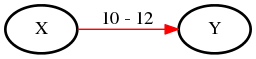
\includegraphics[width=\textwidth,height=0.5in,keepaspectratio
]{ejemplo1.png}\newline
\textit{ejemplo representado como digrafo donde cada nodo representa a una ciudad y la arista hacia donde parte el vuelo desde la ciudad en la que me encuentro.Ademas en la arista se detalla la hora de salida y llegada. Con rojo se indican los vuelos que debo tomar para resolver el problema.} \newline

Se desea llegar de X a Y y se provee de un vuelo. El mismo se realiza desde la ciudad X partiendo a 10 horas de realizada la consulta y se llega a la ciudad Y dos horas después de la partida. En este caso tengo un vuelo disponible que me permite efectuar el recorrido deseado. Debido  a que es el único, el problema no cuenta con ninguna otra solución posible, de esta manera la solución óptima es aquella que cuenta con el vuelo 1 y el horario de llegada se realiza a las 12hs de la consulta.\newline \newline


Ejemplo 2:

X Y 2
vuelos:
1) X A 10 12;  2) A C  14 16\newline
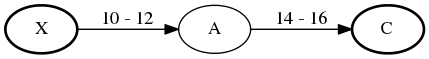
\includegraphics[width=\textwidth,height=0.5in,keepaspectratio
]{ejemplo2.png}\newline

En este caso el objetivo es llegar de X a Y con los dos vuelos disponibles. El primero  se realiza desde la ciudad X a la A . Luego, el otro parte desde A hasta C, el destino de este vuelo es la ciudad C. Como este fue el último de los disponibles, y  no llegue a Y. No hay solución.\newline \newline

Ejemplo 3:

X Y 8
vuelos:
1) Z X 1 5;  2) X A 10 22;  3) A B  24 28;  4) A B 35 41;   5) B Y 42 55;  6) X C 12 18;
7) C D 22 30;  8) D Y 34 40\newline
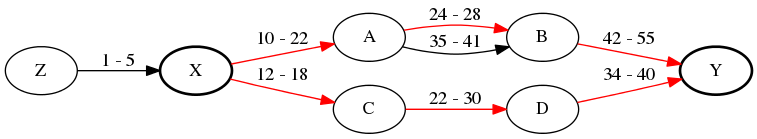
\includegraphics[width=\textwidth,height=\textheight,keepaspectratio
]{ejemplo3.png}\newline


Para llegar a X desde Y existen dos posibles itinerarios. Uno de ellos es el que contiene a los vuelos numero 2, 3, 5 y 6 ya que el tomar los vuelos en este orden me permite llegar a destino. Y entre cada uno de los vuelos se cumple que entre el horario de llegada y salida desde la misma ciudad  
haya dos horas de diferencia. Y el otro itinerario posible, es el de los vuelos 6, 7, 8. Si bien ambas son soluciones, solo el ultimo itinerario es una solución óptima al problema. Ya que, la llegada a Y se realiza 15 horas antes que en el otro itinerario y recordemos que es solución óptima el conjunto de vuelos que llega antes a destino.\newline  \newline


Ejemplo 4:

X Y 14
1) X A 1 10;  2) A C 15 20;  3) C D 22 30;  4) D Y 34 40;  5) D E 32 36;  6) E Y 38 40;  7) X T 1 5;
8) T U 7 15;  9) U V 21 25 ;  10) U D 20 28;  11) V W 27 30;  12) W Z 32 35;  13)  Z S 37 41;
14) Z Y 38 40  
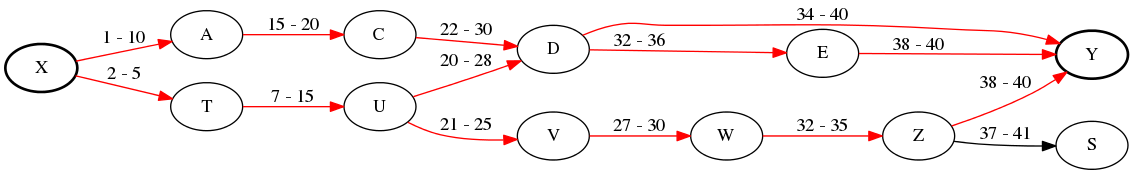
\includegraphics[width=\textwidth,height=\textheight,keepaspectratio
]{ejemplo4.png}\newline

Para este ejemplo contamos con un total de 13 vuelos. Y el objetivo es dar una solución óptima al problema de llegar desde X hasta Y. Una posible combinación de vuelos, y por lo tanto un itinerario factible, es el de los vuelos 1, 2, 3 y 4. Pero, no es el único, otro puede ser el de los vuelos 1,  2, 3, 5 y 6. También esta el que contiene a  7, 8, 9, 11, 12 y 14. y por ultimo el de los vuelos 7, 8, 10 y 4. En este caso tengo 4 itinerarios que cumple la necesidad de llegar a destino a partir de X. Edemas se puede observar que solo hay tres vuelos que llegan a destino el numero 5, 6, 14. Pero estos tres llegan a la misma hora. Entonces cualquiera de los 4 itinerarios es una solución óptima al problema.\newline \newline





{\noindent \Huge Resoluci\'on:} \newline \newline


Como el objetivo del problema es ir de una ciudad $origen$  a una ciudad $destino$,  llegando a la misma en el menor tiempo posible y devolviendo los vuelos utilizados (se devuelven los vuelos enumerados por orden de aparición en la entrada). Teniendo una cantidad $n$, entero no negativo, de vuelos disponibles, donde cada vuelo esta constituido por dos string $lugar\_de\_salida$, $lugar\_de\_llegada$. Lo que se va a realizar en primera instancia es a cada ciudad distinta asignarle un numero entero (esto se realiza para mantener la complejidad deseada),  de esta forma me van a quedar ciudades enumeras de 0 a 2*n-1 (en el peor caso, si cada vuelos tiene ciudades distintas entonces tengo 2*n ciudades). Luego, como se desea ir de $origen$ a $destino$ se verificara que estas ciudades existan entre los vuelos disponibles. Si alguna de las dos no existe, entonces no hay solución, no puedo partir o llegar desde las ciudades deseadas. En caso contrario se ordenaran los vuelos de manera decreciente por $hora\_de\_llegada$ y se creara un vector de listas $donde$, donde las posiciones del vector representaran a cada ciudad (ciudad mapeada a un entero) y las listas en cada una, la posición según $vuelos$, donde esta ciudad es un $lugar\_de\_salida$. Un arreglo de enteros, $vuelos disponibles$, donde cada posición es una ciudad y el valor entero en dicha posición es la cantidad de vuelos que hay donde dicha ciudad es un $lugar\_de\_salida$ entre los vuelos disponibles. Y finalmente un arreglo de bool $ya\_lo\_use$ como cada vuelo puede ser numerado apartir de la posición que se encuentra en $vuelos$ este arreglo me va a servir para informar si ya analice un camino para llegar a $destino$ a partir de tomar el vuelo que se este analizando, por lo que inicialemente $ya\_lo\_use$ tendra el valor false en todas sus posciones. Luego de estas estructuras auxiliares se va a proceder a ver si existe alguna combinación entre los vuelos que me permita cumplir con el objetivo. Primero, se verifica que haya vuelos disponibles para la ciudad $origen$, si es igual a cero entonces no hay. Por ende, no hay solución. Sino, se verificara por cada vuelo que parta desde la ciudad $origen$ si tomando ese vuelo existe alguna combinación que me permita llegar a $destino$ realizada la verificación, se procede  a almacenar la posible solución en una lista, y se procede a realizar los mismo con el siguiente vuelo que parta desde $destino$ hasta el último que haya. La verificación se realiza con la función  $buscar\_llegada$ la misma consta de $vuelos$, $donde$, $destino$ $vuelos\_disponibles[]$, $numero\_de\_vuelo$, $ya\_lo\_use$ y el vuelo actual que es el que parte de $origen$.
Esta función primero va a corroborar que si la ciudad de llegada del $vuelo\_actual$ es destino entonces llegue a donde quería y retorno como solución la hora de llegada y el numero de vuelo, primera y segunda componente de una tupla respectivamente. Si no es así. Se verificara si existe un vuelo a partir de la ciudad de llegada de $vuelo\_actual$ que me permita llegar. Si la cantidad de vuelos disponibles para esta ciudad es cero. Entonces no llegue a destino, y ya no tengo mas vuelos para seguir, se devolverá como solución el valor -1 y una lista vacía. Si hay vuelos disponibles entonces se verificara si tomando los vuelos que salen desde esta ciudad de llegada. Puedo llegar a $destino$, es decir se llamara recursivamente a la función $buscar\_llegada$. Pero, antes de llamar a esta función se verificara que haya una diferencia de dos horas entre la hora que llego a la ciudad y el próximo vuelo que parte de esta y que no se haya trabajado con este vuelo. Si hay varios vuelos que parten de una misma ciudad y cumplen con estas condiciones, se tendrán varias soluciones dependiendo del vuelo que tome. Entonces, a cada solución se la almacenara temporalmente en una lista y se va a decrementar la cantidad de vuelos disponibles para la ciudad de la que parti en uno. Y se denota como true a la posicion de $ya\_lo\_use$ para este vuelo. Cuando se terminen de recorrer todos los vuelos. Tendré una lista con posibles soluciones. Si en cada posible solución el valor de la primer componente es -1 significa que no llego a destino con esa combinación de vuelos. Si hay alguno que no lo es, devuelvo el de menor valor. Eso significa que llegue a $destino$ y como me interesa el que antes llegue devuelvo eso.
Finalmente al analizar todos los vuelos que salgan desde $destino$ (terminan las iteraciones del ciclo de $desde\_origen$). Verifico que haya solución,si la hay devuelvo la de menor tiempo de llegada. Ahora es cuando se utiliza la segunda componente que contiene los números de vuelos que use. Si bien estos corresponden a los vuelos ordenados tan solo basta encontrar cual es la posición en el vector sin ordenar. Y devolverlos.  


 
\vspace{0.4cm}
\begin{algorithmic}[1]
\Procedure{Desde\_Origen}{$vector<string>$ $ciudades$, $vector<int>$ $horarios$, $string$ $origen$, $string$ $destino$}
        \State $vector<string>$ $mapeados \gets$ $\textit{devolver todas las ciudades sin repetirlas(ciudades)}$
        \State $vector<vuelo>$ $vuelos\gets$ \textit{crear vuelos asignando a cada ciudad su posicion en mapeados($mapeados, ciudades, horarios$)}
        	\If{\textit{(no existe la ciudad $origen$ o $destino$ en mapeados)}}
        		\State \textit{No hay solución}
        	\Else 
        		\State $\textit{ordenar crecientemente por orden de llegada (vuelos)}$
        		\State $vector <list <int> > donde \gets posiciones\_de\_salida(vuelos)$
			\State bool $ya\_lo\_use[vuelos.size()]$ 
			\State \textit{asignar a cada posicion de ya\_lo\_use false(ya\_lo\_use)}       		
        		\State int vuelos\_disponibles[cantidad de ciudades distintas];
        		\For{($i$ = 0; $i$ $<$ cantidad de ciudades distintas; $i_{++}$)}
        			\State $vuelos\_disponibles[vuelos[i].lugar\_de\_salida]_{++}$
        		\EndFor	
        		\If{(vuelos\_disponibles[destino] == 0)}
        			\State \textit{No hay solución}
        		\Else	
       			\State $list$ $<tupla<int, list<int> > >$ soluciones; 
				\State $list<int> vuelos\_desde\_destino \gets donde[destino]$ 		
				\For{($iterador$ $it\gets vuelo\_desde\_destino.begin()$ to $vuelo\_desde\_destino.end()$ }
					\State $posible\_solucion\gets$ buscar\_llegada($vuelos$, $vuelos\_disponibles$, $vuelos[*it]$, $*it$,  $destino$, $donde$, $ya\_lo\_use$)
					\State soluciones.Push\_back(posible\_solucion)
				\EndFor
				\If{(no\_hay\_camino(soluciones))}
					\State \textit{no hay solucion}
				\Else
					\State return(minimo\_camino(soluciones))
				\EndIf
			\EndIf
		 \EndIf			 	
\EndProcedure
\end{algorithmic}

\vspace{0.2cm}
\begin{algorithmic}[1]

\Procedure{Buscar\_llegada}{$vector<vuelo>$ $vuelos$, $int$ $vuelos\_disponibles[]$, $vuelo$ $vuelo\_actual$, $int$ $numero\_de\_vuelo$, $int$ $destino$, $vector< list<int> >$ $donde$, $bool$ $ya\_lo\_use$}
        \State $tupla<int , list<int> >$ $itinerario$ 
        	\If{\textit{(vuelo\_actual.lugar\_de\_salida == destino)}}
        		\State $list<int>$ $camino$
        		\State return $tupla<vuelo\_actual.hora\_de\_llegada, camino.push\_back(numero\_de\_vuelo) >$
        	\Else 
        		\If{(vuelos\_disponibles[vuelo\_actual.lugar\_de\_llegada] !=0)}
       			\State $list$ $<tupla<int, list<int> > >$ soluciones;
       			\State $list<int> vuelos\_desde\_nuevo\_destino \gets donde[vuelo\_actual.lugar\_de\_llegada]$ 		 
				\For{(iterador it vuelos\_desde\_nuevo\_destino.begin() to vuelos\_desde\_nuevo\_destino.end() )}
					\If{(vuelos[*it].hora\_salida - vuelo\_actual.hora\_llegada $>=$ 2 $\&\&$ $!ya\_lo\_use[*it]$)}										
						\State $posible\_solucion\gets buscar\_llegada$
						\State soluciones.Push\_back(posible\_solucion)
						\State vuelos\_disponibles[vuelo\_actual.lugar\_de\_salida]--;
						\State ya\_lo\_use[*it]= true
					\EndIf					
				\EndFor
				\If{(no\_hay\_camino(soluciones))}
					\State itinerario.fisrt = -1
				\Else
					\State itinerario =  minimo\_camino(soluciones)
					\State itinerario.second.push\_back(numero\_de\_vuelo);
				\EndIf
			\Else
				\State itinerario.first = -1
			\EndIf
			\State return itinerario
		 \EndIf			 	
\EndProcedure
\end{algorithmic}

\vspace{0.2cm}
{\noindent \Huge Complejidad:}
\newline \newline

Para calcular la complejidad total vamos a analizar por partes nuestro algoritmo.\newline
1) La funcion principal $desde\_origen$ recibe dos vectores. Uno de ellos de string que representa a las ciudades, $ciudades$ y otro las hora de salida y llegada $horarios$. Como ya se menciono, cada ciudad distinta sera mapeada a un valor entero. Para esto se procede a crear una lista con las ciudades, de manera que en esta no haya ciudades repetidas. Entonces, tendre a lo sumo 2*n ciudades y según la posicion que ocupe cada ciudad sera el numero que se le asignara. El costo de esto, fue crear la lista con las ciudades sin repetidos,  O(2*n) tamaño de la lista. Más verificar no introducir una ciudad repetida para esto, si estoy recorriendo la posicion i-esima de $ciudades$, 1$<=$ $i$ $<$ n,  me fijo si a esta i-esima ciudad no la analice antes, es decir desde la posicion 0 a i-1. \newline
$\sum_{i=0}^{2*n}{i}= O(n^{2})$\newline
2) Teniendo un valor entero que representa a cada ciudad se construye el vector $vuelos$ del tipo  vuelo. A medida que se recorre el vector de ciudades y de horarios, avanzo de a par, la primer posicion de este par en $ciudades$ es el $lugar\_de\_salida$, y el segunda la $ciudad\_de\_llegada$ mientras que en el otro vector representa $horario\_de\_salida$, $horario\_de\_llegada$ respectivamente todo para un mismo vuelo. Pero antes de construir el vuelo las ciudades en cuestion  deben ser con su asignacion al valor entero. Para esto se debe buscar en mapeados la posicion que ocupa la ciudad. Complejidad:
O(2*n) + O(2*n) (buscar por cada ciudad, de vuelo y de llegada, de un vuelo el valor entero que tiene asignado, siendo el tamaño de mapeados a lo sumo 2*n) y esto se realiza para todas las ciudades 0(2*n*(O(2*n) + O(2*n))) = O($n^{2}$).\newline
3) Verificar si existen las ciudades $destino$ y $origen$, se comienza con dos bool en false para indicar si existe cada uno.  Y se recorre la lista $mapeados$ si estan se cambian los bool  de false a true.  Al recorrer toda la lista si alguno de los bool siguen en false no hay solucion. Complejidad: O(2*n).O(1) (recorrer mapeado por el costo de verificar si las ciudades existen, comparar string).\newline
4)    Ordenar el vector $vuelos$ se usa el   sort provista por la stl. Complejidad O(n*log(n)) siendo n la cantidad de vuelos.\newline
5) Crear el vector de listas de int $donde$, mediante el uso de la funcion auxiliar $posiciones\_en\_vuelo$. La misma se encarga de recorrer el vector $vuelos$ y por cada ciudad de salida del vuelo que se este recorriendo guarda en la poscion que le corresponda de $donde$ la posicion de este vuelo en $vuelos$, es decir si estamos en la i-esima iteracion del vector vuelos, 0$<=$ $i$ $<$ n. se guarda el valor i (recordemos que ahora los vuelos son del tipo entero de 0 a 2*n-1, en el peor caso, por lo que cada cada valor se asocia a una posicion). Complejidad : O(n).O(1) (recorrer el vector vuelos por lo que cuesta asinar las posciones que son push\_back en cada lista.)\newline
6) Crear el arreglo $ya\_lo\_use$ que tiene el mismo tamaño que la cantidad de vuelos disponibles. Y a cada posicion hay que asignarle el valor false: O(n) en total\newline
7) Construir el vector $vuelos\_disponibles$, el mismo es de tamaño de $mapeados$ ya que por cada  ciudad quiero indicar la cantidad de vuelos que salgan desde esta ciudad. Por lo que la reslucion es similar al item 5). se recorre $vuelos$ pero ahora en vez de guardarme la poscion incremento en uno el valor de la poscion que represente la\_ciudad\_de\_salida. O(n) (recorrer vuelos el incrementar el valor según el vuelo de salida es O(1)).  \newline
8) verificar que haya vuelos disponibles desde destino, O(1) me fijo si el tamaño de la lista es == 0 en el vector $donde$ y posicion $destino$. usando la instrucción empty() provista por la stl.\newline
9) Verificar si hay alguna combinacion de vuelos que me permita llegar a destino. Como se hace uso de una funcion recursiva, $buscar\_llegada$. Primero vamos a analizar la complejidad de lo que se realiza en cada llamada.\newline
9.a) $buscar\_llegada$ devuelve una $tupla<int, list<int>>$ $itinerario$, la primer componente tendra el horario de llegada si es que hay un camino hacia $destino$ y la segunda el numero de los vuelos que me permiten llegar. En caso contrario solo tendrá el valor -1.  Si llegué, a la primer componente se le asigna el horario de llegada del vuelo actual O(1) , se crea la lista que va a tener a los numeros de vuelo y se pushea $numero\_de\_vuelo$ O(1).\newline
9.b) si no se llego a destino, y la cantidad de vuelos disponibles para la ciudad de llegada del vuelo actual es distinta de cero. Entonces, significa que existen vuelos que parten desde esta ciudad pudiendo que exista la forma de llegar a destino. Se evaluaran todos los vuelos que salgan haciendo tantas llamadas a la funcion $buscar\_llegada$ como vuelos hayan que salgan desde esta ciudad. Los mismos se conocen por $donde$, solo basta buscar a este vuelo en la estructura. Como ahora las ciudades son un entero entre 0 a 2*n-1 con usar donde[vuelo\_actual.lugar\_de\_salida] ya los tengo (este es el principal de uso de tener mapeadas las ciudades a un valor entero, puedo obtener esta información en O(1)). Al ya tener los vuelos que debo analizar se procede a realizar un for que verifique con cada uno de estos vuelos si puedo llegar a $destino$, luego de cada llamada se guardara la posible solución en una lista provisoria. (Luego se realizara un analisis del costo de esta asignacion). La verificacion con los mismos se realizara si cumplen dos condiciones. La primera es si cumple la diferencia de horario (requisito necesario por el problema), la segunda es que, ya no se haya analizado este vuelo porque si se analizo entonces estaria repiento la busqueda que ya analice y es necesario para nuestra complejidad que los vuelos solo se analicen una sola vez. Cuando los vuelos se analizan se disminuyte la cantidad de vuelos disponibles de la ciudad de llegada del $vuelo actual$. Y  en$ya\_lo\_use[numero\_de\_vuelo]$ le asigno true para que si otra combinacion de vuelos hace uso de este, ya se sabe que se analizo y no tener que calcular nuevamente lo mismo. Para poder cumplir con que los vuelos se analicen una sola vez  es que se ordenaron los vuelos por orden de llegada, se tiene el vector $ya\_lo\_use$ y $vuelos\_disponibles$. Ya que el tenerlos ordenados por orden de llegada da mayor probabilidad de que el vuelo $t$ que este analizando sea el primero en llegar a una determinada ciudad. Entonces, si este cumple con la condicion de horarios voy a poder analizar todos los vuelos que salgan de esta ciudad y la cantidad de vuelos disponibles para la posicion $t.lugar\_de\_llegada$ va a ser igual a cero. Por lo que si hay otros vuelos que luego utilicen a $t$ como vuelo de esacala, al verificar si hay vuelos disponibles tendran que no, (que es igual a cero). De esta forma me aseguro de no realizar analisis repetido. Ahora bien, puede que el vuelo que este analizando no cumpla con la diferencia horaria para todos los vuelos pero si para algunos, es por eso que ademas se cuenta con $ya\_lo\_use$. Para los vuelos que se puedan verificar entonces se los verificara y se tendra marcado que ya los revisaron asi los posterior vuelos no necesitan volver a revisar estos sino, aquellos que en su momento no se pudieron hacer por no cumplir la diferencia horaria.  Luego, de tener para la instancia de vuelo $t$ todas las posibles soluciones se procede a verificar si hay solución y si la hay, cual es. Para esto primero se verifica que todas las posibles soluciones no tengan el valor -1 en su primer componente si es asi entonces no hay solucion y se devuelve la tupla creada al principio $itinerario$ con el valor -1 en su primer componente. En caso de que la haya se recorre todas las soluciones y se devuelve el menor valor distinto de -1 ambas funciones son lineales en la cantidad de posibles soluciones, y esta cantidad es igual a los vuelos que parten desde $t$.lugar\_de\_llegada. La suma de todos los vuelos disponibles debe ser igual a n, ya que son todos los vuelos que existen. Como se analizan por cada iteracion del ciclo de $desde\_origen$ a lo sumo una vez cada vuelo y luego si se necesita de un vuelo verificado con ver la canidad de vuelos disponibles o si ya fue usado basta, con complejidad O(n) en el peor de los casos, todos los vuelos necesitan verificar esto, por cada vez que se realiza una iteracion en  $desde\_origen$ en el peor de los casos se pregunta c veces (c son los vuelos desde $destino$) entonces seria c.O(n) acotando c por n tenemos O($n^{2}$). \newline
9.c)Finalmente analizamos la complejidad de las asignaciones hechas. Cada vez que analizamos todos los buenos de una ciudad se guardan en una lista provisoria el resultado de llamar a $buscar\_llegada$ con uno de los vuelos que parten desde esta ciudad. Al guardar esto, si bien se utiliza la funcion push\_back(), se esta guardando una tupla que posee una lista de los vuelos usados para llegar a $destino$ si es que hay camino sino solo una tupla con una lista vacia y esto se hace en O(1). En el otro caso es lineal a la cantidad de elementos en la lista. Entonces como cada vuelo se analiza a lo sumo sola vez, en todas las iteraciones estaremos realizando copias con valores distintos. No podria haber como solucion un vuelo que este tambien como solucion para otro camino ya que cuando se lo analizo por primera vez se puso que ya fue usado este vuelo en $ya\_lo\_use$ y en este caso nuestro algoritmo plantea que no hay solución porque ya se analizo este vuelo y ya se conoce su resultado . Entonces, si al finalizar todas las iteraciones de $desde\_origen$ se tienen k posibles soluciones, (k igual a los vuelos disponibles desde $destino$). Significa que tengo k listas que fueron copiadas tantas veces como vuelos se necesitaron para llegar a $destino$. Suponemos el peor caso que todos los vuelos llegan a destino entonces la suma de las longitudes de esas listas es n, (por lo argumentado anteriormente no se utilizan vuelos que hayan en otras soluciones). Entonces, si pensamos ahora todo como una sola lista y suponemos que fue copiada tantas veces como la máxima vez que fue copiada algunas de las k listas. Y sabemos que las listas se copiaron a lo sumo n veces porque se van insertando de a uno cada nuevo $numero\_de\_vuelo$ 
tenemos que la complejidad de todas las copias son:\newline
$\sum_{i=0}^{2*n}{i}= O(n^{2})$\newline
\textit{cada vez que voy a agregar un nuevo elemento copio todos los anteriores}\newline
9.d)Luego, se procede a verificar cual de las k soluciones es la correcta, utilizando nuevamente si existe solucion y cual es, ambas lineales en la cantidad de posibles soluciones O(k), acotando k por n tenemos O(n)\newline
juntando las complejidades de los casos 1-9 tenemos que la complejidad total es:     

$O(n^{2})$ + $O(n^{2})$ + $O(2*n)$ + $O(n*log(n))$ + $O(2*n)$ + $O(n)$ + $O(2*n)$ + $O(1)$ + $O(1)$ +$O(n^{2})$ + $O(n^{2})$ + $O(n)$  = $O(4*n^{2})$ + $O(2*n)$ + $O(2)$ + $O(n*log(n))$ + $(3*2*n)$ = $O(n^{2})$ + $O(n*log(n))$ =  $O(n^{2})$
\newline\newline
{\noindent \Huge Experimentaci\'on:}
\end{document}